\documentclass[UTF-8,openright]{ctexbook}

\usepackage[sectionbib]{bibunits}
\bibliographyunit[\chapter]
\defaultbibliographystyle{thuthesis-numeric}
\defaultbibliography{main}

\renewcommand\bibname{\centerline{参考资料}}

\usepackage{graphicx}

\usepackage[colorlinks, linkcolor=black, anchorcolor=blue, citecolor=green]{hyperref}

\begin{document}

%\title{清华园第四年}
%\author{张丹阳}
%\date{}
%\maketitle

\begin{titlepage}
	\centering
	\linespread{1.2}
	\vspace*{1cm}
	{\zihao{-0} \textbf{清华园第四年}\par}
	\vspace{0.5cm}
	{\zihao{-1} \textbf{——清华园怪谈集}\par}
	\vfill
	\begin{table}[!hb]
		\LARGE
		\centering
		\begin{tabular}{rc}
			作者: &	张丹阳 \\
			&			程思源 \\
			取材: &	程思源 \\
			&			张丹阳 \\
			摄影: &	程思源
		\end{tabular}
		\vspace{1cm}
	\end{table}
\end{titlepage}

\pagestyle{headings}

\pagenumbering{Roman}

% TODO: 初版前言

\tableofcontents
\newpage

\pagenumbering{arabic}

\chapter{序章}

眨眼间我在清华园已度过了三年。
三年我吃过了园子里11个食堂,出入过4个图书馆,踏遍了6个教学楼,还借着阿甘跑步的时候跑遍了各种各样的小角落,自以为已对清华园非常熟悉了解。
然而,第四年,我却惊讶地发现,园子里还有这么多地方,我未曾踏足……

\vfill

\paragraph{记事}
2020年由于突发的疫情,在家里困了一个学期,6月份终于允许毕业生返校。
笔者毕业后就要去其他学校读博了,因此这本来是能够留在园子里的最后一个学期,只是如今仅剩下寥寥的数周了。
此番离去,之后回来的机会便少了许多。为了能够多留下些回忆,笔者约了朋友C君再在最后离校前逛一逛清华园。
晚上走在人迹罕至的小路上,就会有一种微妙的紧张与刺激感,于是便和C君聊起了魑魅魍魉、月黑风高的事情,谈笑间产生了杜撰些怪谈的想法。
笔者文笔枯燥乏力,实在缺乏表现力,本来只当个玩笑,但终于还是决定写下来,权做四年清华生活的纪念。
此间故事,皆为杜撰;怪力乱神,洵有其缘;茶余闲谈,供君一笑耳。

% 简要提纲
% 
% 1. 素材
%    * 荷塘南面,西湖西北,小山上,月黑杀人夜,风高放火天,零零阁
%    * 荷塘仿若小提琴声的荷香,荷仙的歌声,荷塘月色
%    * 装满水的西湖,服务看不见的客人
%    * 荷塘东侧的小山
%    * 夜晚的工字厅,门口的灯,冥府之门
%    * 苏世民书院后的凉风
%    * 二教的地下室,不开放自习,旧人体实验室
%    * 大礼堂后的小径,限时开放,大礼堂的地下室


\chapter{零零阁}

在荷塘南面,西湖北面,有一座小山。西边的山头上,有一座高大的阁子,唤作零零阁。%据说是以前“零零字班”的校友捐建的,因此得名。
1970年,适逢清华园学制由6年改为5年,两个年级的学生在同一年毕业。
当时校内习惯以毕业年份来作为届号,故早一年入学的称为“零字班”,晚一年入学的便称为“零零字班”。
这座阁子,便是由零零字班的校友捐建的。
阁子有两层,有着高高的螺旋台阶,矗立在山顶上,是这一范围内最高的建筑物,可以一览原来的皇家园林的秀美景观。

\begin{figure}[!b]
	\centering
	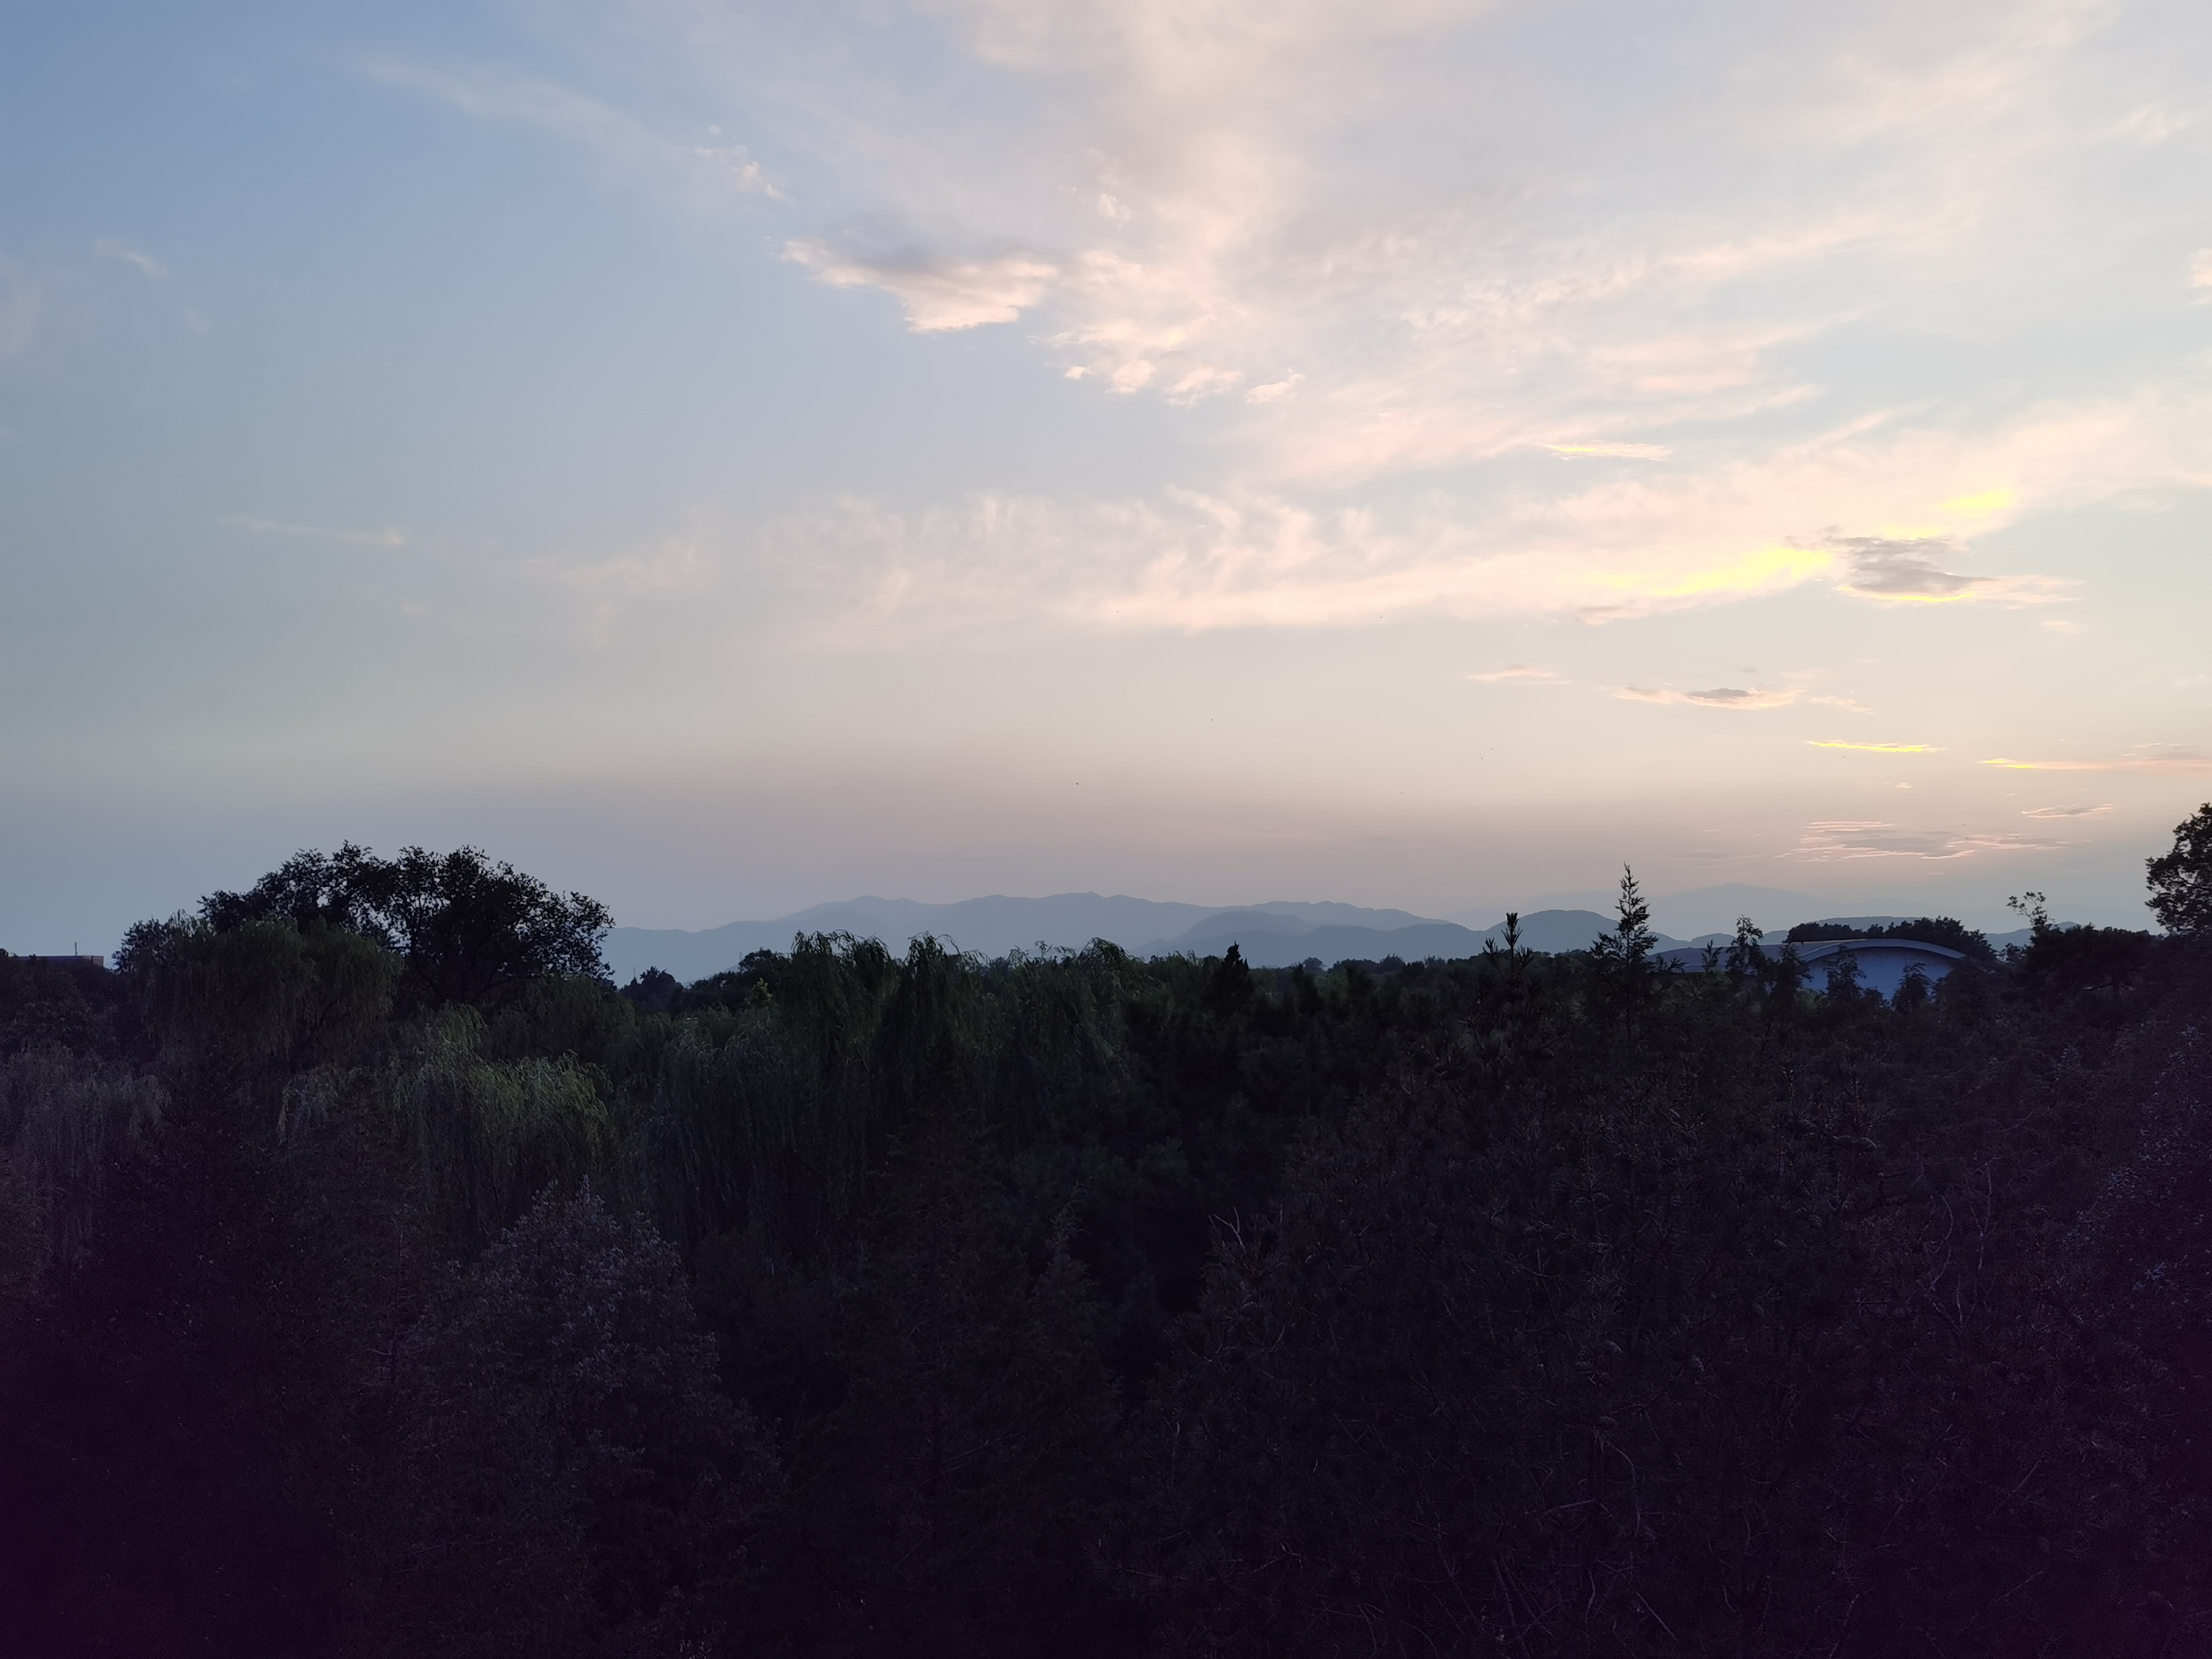
\includegraphics[width=\linewidth]{figures/零零阁暮望西山.jpg}
	从零零阁上远望西山。
\end{figure}

之前我与C君曾在阳光长跑时到过这个亭子。
当时跑得随性,只记得路过西湖附近,发现山上隐约有个亭子,便寻得路登了上去。穿过树丛,一座高大的亭子便豁然闯入眼帘。
我们正跑得气喘吁吁,然而登上二层后,阵阵凉风袭来,不胜清爽。
视野也陡然开阔。悠然东望,能从翠绿掩映中寻得六教深红的一角;极目向西,则甚至望得到远方巍巍西山:一时竟有种“一览众山小”的豪迈感,仿佛胸怀也随之变得更豁达了。
我们都对当时的场面印象深刻。于是C君提议,今日再登一次零零阁。

然而我们都已不记得这阁子的具体位置了,只大致记得应该是在荷塘旁靠近西湖的地方,于是我们便直奔荷塘而来。
荷塘北岸一马平川,自不可能有什么山巅的阁子。而湖心岛转过一遍,也没有发现符合当时印象的双层亭阁。
于是我们向荷塘南岸寻来。

荷塘这里靠近生活区,平时晚上就有许多人来这里散步、活动,因此相比园子里其他地方,有着浓浓的市井气息,仿佛城市里的公园一般。
然而晚上出来散步的人都聚集在荷塘北岸以及湖心岛的西北角,东面和南面的人烟便十分稀少,沿岸行走的话,仅间或能看到一两个默默垂钓的人。
我们沿荷塘东岸向南,至莲桥再向西。一过莲桥,就察觉这里人气已淡了许多。
太阳已经落山,又是阴天,浓云蔽月,再添上南岸茂密的树林,这时走在幽黑的林荫小径上,一阵凉风吹过,竟觉得有一些阴冷。
越向里走树木就越发茂密,光线也越来越暗,小径就仿佛没有出口的黑洞般,一直走不到尽头。这时我看到旁边有一条曲折延伸到山上密林中的小路。
微风吹过,我在这盛夏时节也不禁微微打了个寒颤,然后指着拐出去的小路说:“那亭子应该是在山顶上,我们一直沿着湖岸走要走到什么时候,不如往这里上去找一找。”C君亦以为然,于是我们便向山上走去。

\begin{figure}[!h]
	\centering
	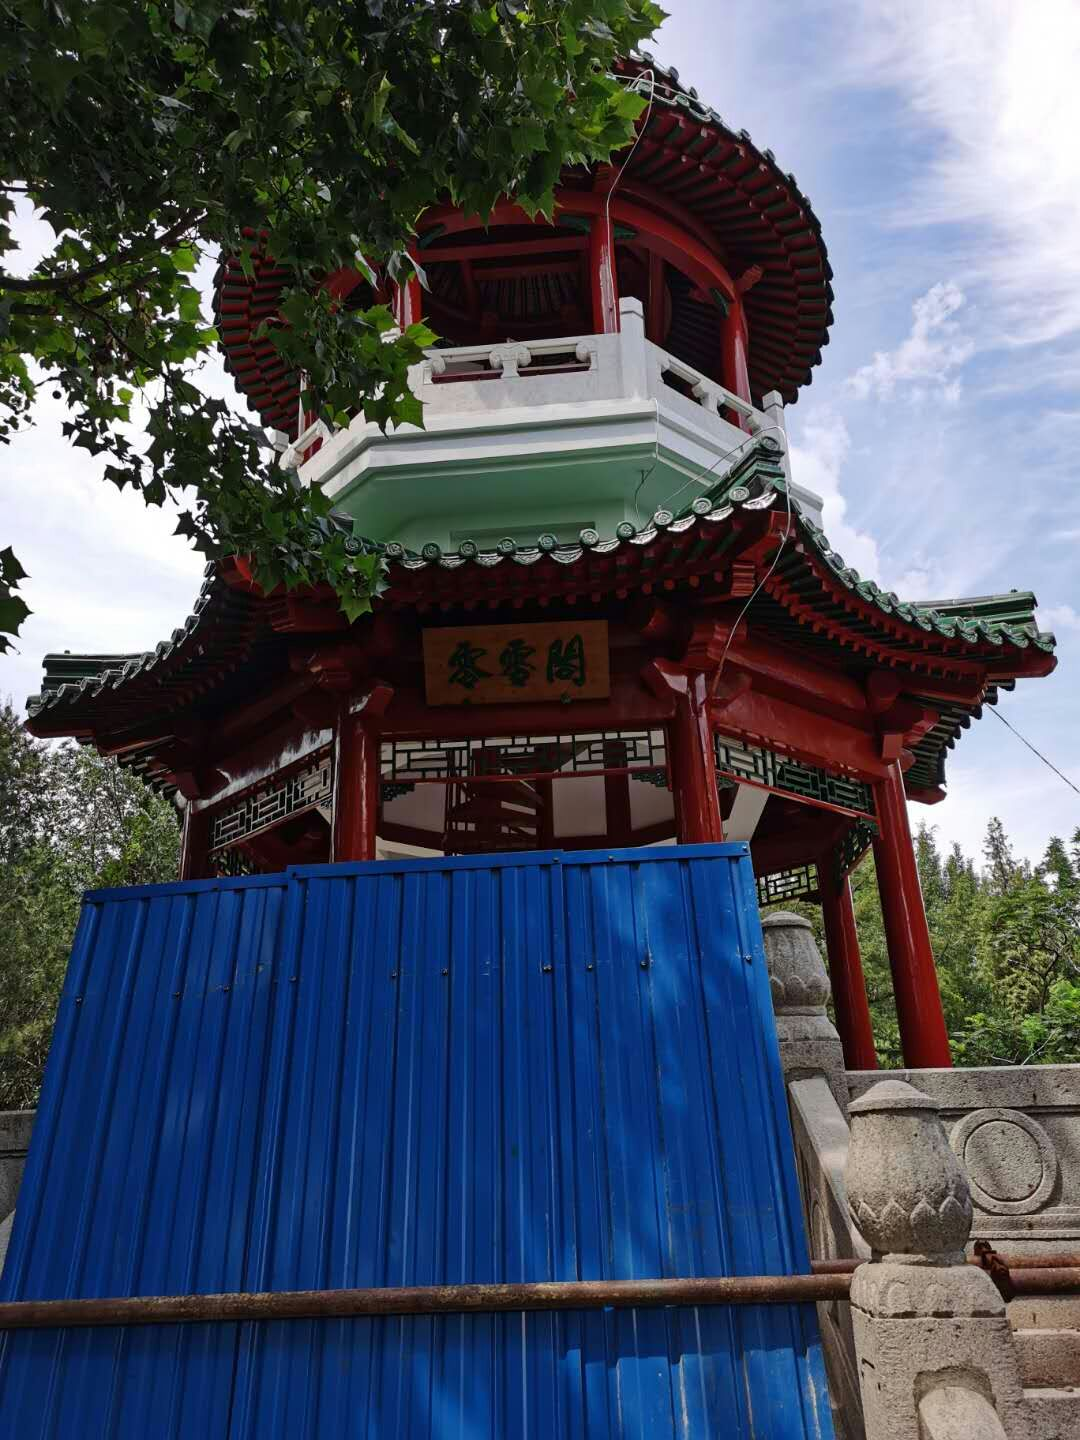
\includegraphics[width=\linewidth]{figures/零零阁.jpg}
	零零阁
\end{figure}

上山的小路坑坑洼洼的,许多铺路的石块都缺失了,表面还散布着细碎的石子,给人久未维护的感觉。
靠近山顶,树林稍稍稀疏了些,能够看到天上的阴云,也能看到前方朦胧的建筑,零零阁就在眼前了。
我们喜出望外,急忙沿着山路跑到了尽头,来到了心心念念的零零阁前,却惊讶地发现山路被围挡折断,亭子已整个被包围在其中,显然是正在翻修,无法再上去一瞰清华。大失所望之际,我们也只好再折返下山去。
这时一阵风穿过树林,发出尖锐的啸声,我们俩不禁又打了个哆嗦,不觉间已加快了下山的脚步。

就要走出湖边的小道时,迎面走来了一个满身酒气的人。
小径狭窄,几乎容不下他踉跄的步伐,我们只好赶紧闪到路边草坪上,让他先行过去。
兴许是刚刚赴完局,打算饭后找个清静少人的地方散散步,消消食,醒醒酒,随后便回家去,所以他也不顾夜色已深,便晃悠悠地走进了林荫小道,向荷塘南边走去。
素不相识,他的事,自然与我们无关,因而我们出来后,找到自己的自行车,便匆匆离去了。
当晚无事。

然而三天后的中午,C君突然急匆匆地找到我,递给我一份当日的报纸。
我低头一看,已下子就被报纸上的一条消息吓到了:
“昨日北京市某大学校内小山上某施工地点附近发现一具无头男尸,死状凄惨,全身血液流失殆尽。
法医初步鉴定死亡时间为两天前凌晨时段。
目前案件正在进一步调查中。”
报上黑白的配图虽然有些模糊,但我还是立刻就认出,那正是零零阁所在的那座小山……

\vfill

\paragraph{记事}
6月23日傍晚,笔者约C君出来共游校园,途中C君提到想再上一次零零阁,于是二人往西湖与荷塘这边寻来。
寻觅良久,终于在荷塘南边的小山上找到了亭子,却发现亭子已被围起来翻修了,失望而归。

\chapter{荷塘月色}

报纸上的消息着实令我受到了惊吓,我急急寻得C君交流此事。一交流,才幡然想起,关于荷塘还有着一个危险的传说。

\begin{figure}[!b]
	\centering
	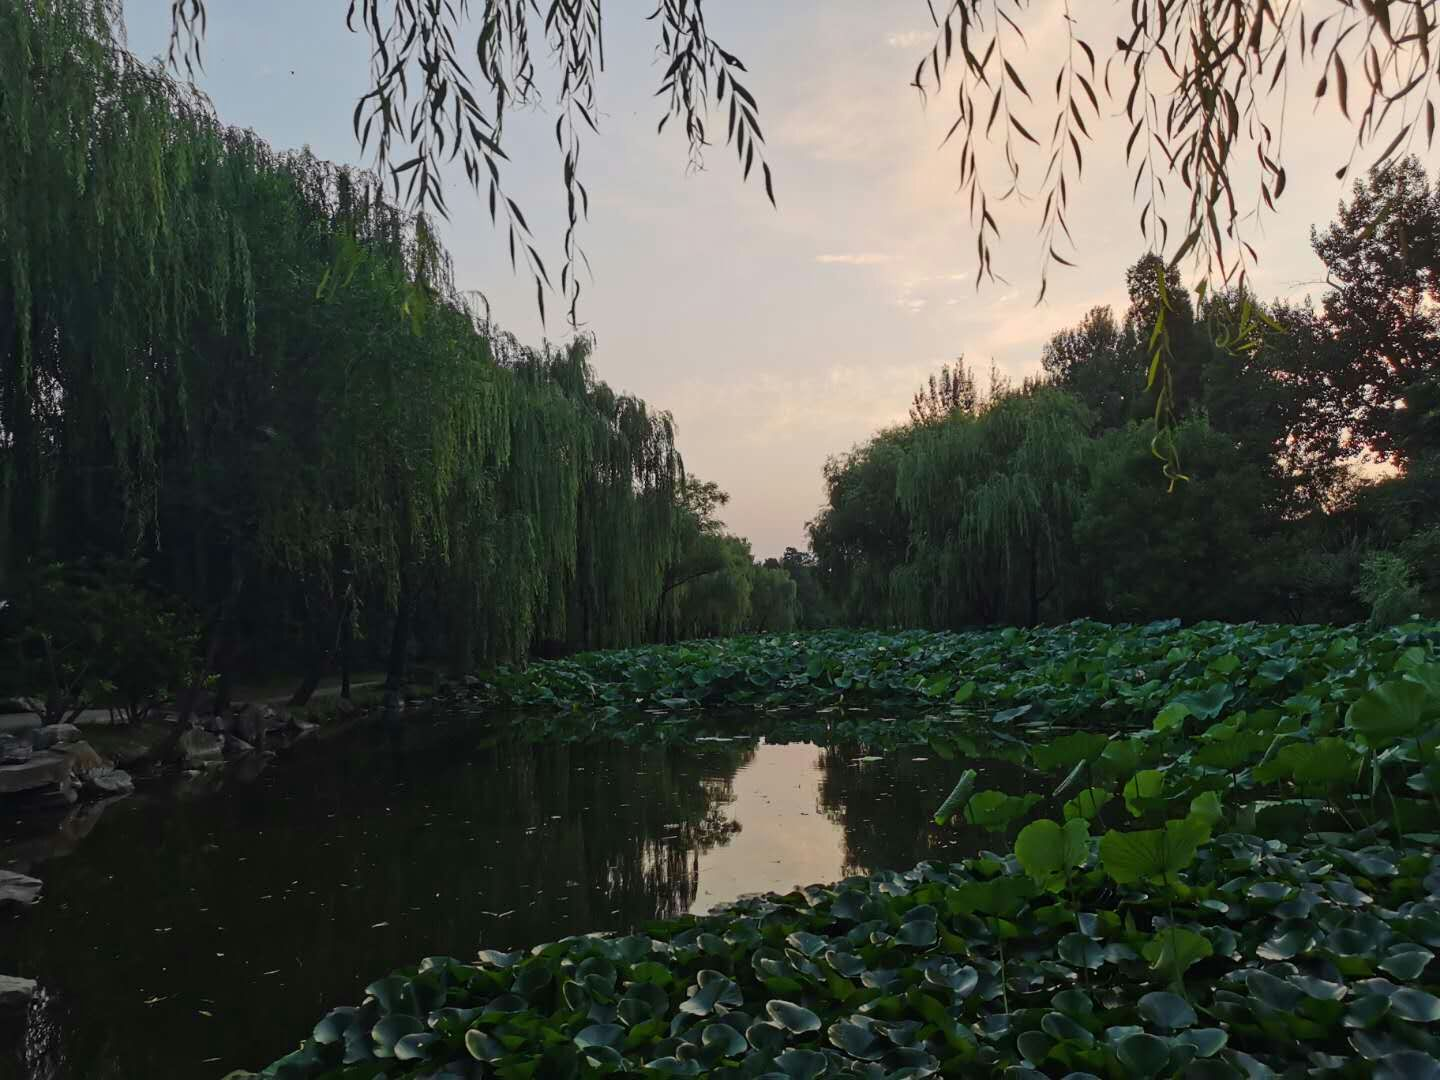
\includegraphics[width=\linewidth]{figures/暮中荷塘.jpg}
	暮中荷塘
\end{figure}

相传荷塘的荷花不是普通的荷花,而是通过美貌与幻音蛊惑行人的荷仙。
白日里,荷塘和其他的莲池并没有什么不同的地方,水面一片清圆,莲花亭亭玉立于碧叶之间,粉嫩白皙,宛若下凡的仙女,妩媚却又神圣。
但当夜色降临,时间逐渐逼近午夜,本应渐归沉寂的荷塘又会热闹起来,一朵朵莲花竟化作了美丽的舞女,荷仙的午夜晚会开始了。
她们的歌声带有魔力,恰如希腊神话中的塞壬,迷人心魂,听者皆会在不知不觉间进入幻境。
她们身形曼妙,舞姿绰约,月色中,树影下,光影迷幻,仿佛梵婀玲上婉转奏着的名曲。
若是恰逢水面上升腾起些许雾气,远远望去,舞池如同隔了一层薄纱,仙子们的身影更加朦胧。醉心观赏时,恍若在悄悄欣赏着远方高楼上渺茫的歌声,逐渐陶醉其中。神游中更好像嗅到了仙子们身上独有的莲香,撩拨着观众的欲望。

本来,我们或许永远都不会知道,在这荷塘中还有这样的聚会。
但是90多年前,一位正处在迷茫中的学者,恰在夜间散步时误入了此地。沉醉在荷仙的歌声与舞蹈中,他很快陷入了神游。在恍惚间他已远离了荷塘,很快回到了自己门前。
从荷塘脱身后,他提笔记下此事,人们才初次了解到,在荷塘还有这样一个不属于人类的世界。

并不是每一个在午夜到过荷塘的人都能如此幸运地全身而退。
这位学者到访的那晚,正值满月,透过薄云,朦胧的月色实在美妙,荷仙们心情正好,或许正是因此,仙子们并没有为难于他。
然而月有阴晴圆缺,据说当月光彻底被云遮住或是恰逢朔月之时,仙子的舞池失去了光源,黑暗中舞会难以举办,烦躁的荷仙便会借路过此地而打扰了聚会的路人撒气,吸其精气,啖其血肉,啮其骨髓。
而我们去寻零零阁的那晚,即醉酒男子进入的那晚,恰是五月初三,又是阴天,本就晦暗的如钩月彻底挡在了阴云之后,是个真正的月黑杀人夜。
想到这里,我们不禁生出了一身冷汗,叹息那醉酒男子的同时,也暗自庆幸,自己没有在池边徘徊,上山寻得阁子后便及时下山离开,脱得险地。

\vfill

\paragraph{附注}
本章故事的创意,皆启发、化用自朱自清先生的《荷塘月色》。

\chapter{西湖魅影}

在近春园荷塘的西南侧,建了个“西湖游泳池”。
平常的年份里一到夏天,这里都非常热闹,许多人来这里游泳;到了冬天则会放水制冰,开辟出一块用作溜冰场;此外听说还有冬泳队的会在这里训练。
然而疫情期间学校里实在是没什么人,印象里往常到游泳、溜冰的人变少的时候,西湖便不再对外开放了,泳池中也不再蓄水,然而那天路过西湖,却发现泳池中装满了水,深感疑惑,于是趁闲时约了C君同往一探究竟。

% TODO: 多搞点环境描写
这天傍晚,吃过晚饭后,我就和C君一起来到了西湖外面。
西湖西侧不远就是近春路;南侧则是清华路;东侧挨着一条小渠,隔渠相望是树木葱郁的小丘;北侧临山,山上就是前几天刚去过的零零阁。泳池四周用铁栏杆方方正正地围了起来。
前几天的命案和荷仙的传说还令我们俩十分忌惮,因此我们也不敢太向山林深处走,只是贴着泳池的围栏走动、观察。

我们沿着西湖边界转了一周,发现大门紧闭,整个泳场空无一人,静得可怕。那诡异的满池清水,也寂静得没有一点波纹。这里似乎除了树上间或传来的两声乌鸦叫和清华路上偶尔经过的行人,便再无一点生气。
天色也渐渐暗了下来,远处荷塘那边似乎传来了人们哼曲唱歌跳舞的乐声,然而这里却仍是一片死寂。
我们转了又转,也还是没有什么发现。这时我脑中突然闪过一个想法,想要鼓动C君一起翻越栏杆进去看看,但思索了一下,还是果断打消了这个想法,一来有些危险,二来若是被发现了,不知会有什么后果,最后一年实在不值得为这事背上一个处分。既然放弃了进一步探索的想法,我便打算和C君一起回去。

然而就在这时,泳池中似乎传来了什么拨动水的声音,我们急忙望去,发现原本平静的湖面上不知为何荡起了一连串波纹,像是小船划过一样,可我却没有在水上看到任何东西。
“那里有什么东西吗?”我悄悄地问C君,然而C君只摇了摇头,表示他也什么都没看到。“不会吧……这是闹鬼了吗?”我有些发怵。
水中的那个看不到的东西似乎还在游动,在水面上留下一道长长的痕迹。
那透明之物游了一会儿,又回到了岸边,随后池边原本干燥的地面上就被洒湿了一片,还能听到湿脚踩地的水声,看来它上岸了。
水留下的脚印开始向泳池南面延伸,一直到了泳池的最南沿,它又拐向西,然后一直走到正门那里,停了下来。
过了一会儿,池塘的南侧突然溅起许多水花,还伴随着入水的声音,紧接着就看到水面上涌起了朵朵浪花,划出了条条波痕,仿佛许多人竞速游泳一般。
夜幕已完全降临,远方的乐声不知不觉间已消失得无影无踪,我们渐渐无法再看清水面上的情况,只听得到池塘中不断地传来划水击浪的声音。
今天实在是开了眼界,我和C君对视一眼,都看出了对方眼中的惊惧,不由得默契地露出了一丝苦笑,随后便悄悄地从南边的清华路上离开了。

\vfill

\paragraph{记事}
6月23日傍晚,与C君寻零零阁途中,路过西湖边,发现西湖泳池中装满了水。由于疫情期间学校应该没有人使用泳池,感到非常疑惑。

\chapter{工字厅}

当晚我们离开西湖时,时间已近深夜,于是我们准备直接返回寝室。
骑车从工字厅前路过时,我们发现工字厅大门前还亮着灯。昏黄的灯光照射在紧闭的红色大门上,显得格外诡异。
看到这种景象,我不由得想起以前看过的一个鬼故事。
说是故宫即使在昼长夜短的夏季也要在下午5点之前就闭馆,原因在于,日月开始交接之后,天地间阳气渐稀,阴气渐盛,一些白日里不敢见光的东西就会开始出来活动。
而故宫作为明清两代的皇宫,四百多年来前廷后宫之中不知发生了多少冤疑悬案,于是一到黄昏时分,出来活动的厉鬼冤魂想来是不计其数,因此为了游客的安全,故宫总要保证在太阳落山之前就要闭馆谢客。

本着不能只有我一个人担惊受怕的想法,我把这个鬼故事讲给了C君,结果C君竟回敬了我一个关于工字厅的鬼故事。
鉴于我们平时就生活在清华园内,这样一个故事某种程度上更加惊悚。

据说那时工字厅门前还不在夜里点灯。
有一次,某位老师下班后又加了很久的班,等他忙完要离开时,天已经完全黑了。
他匆匆收拾好东西就出了门,准备离开。要去开车时,他发现自己竟把车钥匙落在了办公室中,于是又回去拿车钥匙。
然而他这趟回来,跨进工字厅的大门后,却发现原来的办公室不见了,门后是一个从未见过的世界。
一排排硬山顶的传统民房沿几条平行的街道排放,稍远的地方还有二层、三层的阁楼,有些楼下还搭着台子,台子上说书的、唱曲的、献舞的都兴奋地表演着。
街上户户灯火通明,好不红火!
大街上满是没见过的奇奇怪怪的人,有人带着奇怪的面具,有人竖着狐狸耳朵,还有人用袍子将自己整个罩住,只露出一张脸。
虽然各种奇奇怪怪的人都有,但所有人都说笑着在街市上游玩。
街道两旁有卖小吃的,烧鸡酱鸭卤鹅,羊腿猪耳臭豆腐,烧饼凉粉水馒头,各色齐全;
还有各种各样的小玩意儿,没有风也能转的风车,自己发光的石头,变大变小的帽子,无奇不有。
街上人头攒动,除了逛着玩的,还有跑出店来拉客的,殷勤地向游人发放着大红纸印制的广告,诉说着店里的各种妙处。
他愣了一下,急忙要退出来,就发现一个身影飞快地从自己身边飞过,穿出大门而去了。
他不禁吓了一跳,抬眼一看,才发现原来还有人飞在空中。
空中飞着的人身影显得有些缥缈,有些透明,似实似幻,仿佛下一秒就会消散一样,而且越向下接近脚的地方就越透明、越模糊,许多人的脚如果不定睛仔细去看,就已完全看不到了。
再向远方的空中去瞧,隐约间似乎有个岛浮在空中,只是仿佛隔着一层雾一样,实在是看不真切。
这位老师此时已深切地意识到,自己这次是闯入了别人的世界,心中不由得紧张起来,不知道自己还能不能平安回去。想到刚才穿门而出的飞灵,他也不由得猜测这门便是联通两个世界的通道。
想罢,他便赶紧仍从大门退出去,发现工字厅果然还是那个工字厅,清华园果然还是那个清华园;
心中有了点底气,抱着试一试的心态,他再一次跨进大门,果然还是那个光怪陆离的异世界,再退出来,便仍旧是深夜已临的清华园。
这道门,确实已变成了现世与另一个世界的通道。
这位老师心中颇有些感慨难以言明,无处抒发,只是忙从旁边的小侧门绕进工字厅取了钥匙走人了,并暗自发誓从此再也不在工字厅加班。
而就是从这之后,夜里工字厅门前点起了灯,老师们出入也开始只走旁边的小门。
坊间传闻是这位老师在校务会上提出了此事,于是本着对怪力乱神敬而远之的想法,工字厅形成了这样的惯例。

C君讲罢之时,我们正好骑到二教旁边。
二教平日里便不开放自习,深夜更是整座楼都黑不隆咚的,如今外面还围了一圈围挡,更是显得凄凉。
受这氛围所动,我又一下子联想起流传甚广的二教鬼故事,身上不禁升起一阵恶寒,于是催促C君迅速离开了这片是非之地。

\vfill

\paragraph{记事}
6月23日,笔者与C君寻得零零阁后,准备去紫操再叙。骑车途径工字厅,发现工字厅大门在晚上还亮着灯。灯光昏黄,显得有一点点阴森和神秘。

\chapter{第二教学楼}

%\renewcommand\thefootnote{\roman{footnote}}

清华园目前有六个公共教学楼,其中一教、二教都位于早期建筑群处。

% TODO: 来张图瞧瞧

越老的建筑,常常就有越多的迷,二教也不例外,这栋楼几乎是园子里故事最传奇的地方。
二教远离宿舍区和现在以三四五六教为核心的教学区,虽说往常白天的时候也有许多游客,但游客也不会进入教学楼,因此其实没有什么人气;
而且二教不开放自习,没课的时候也就显得格外冷清。
不过由于楼内都是大教室,因此有课的时候二教的教室也显得比别处的教室空旷;
又开着空调,即使是酷暑,在二教里也会觉得冷。当然这一点上,六教也差不多,冷气开得一个比一个足。

二教最让人不解的地方莫过于教室的编号和分布了。
这里教室的楼层号并没有单独编号,而是顺着一教往下编的。一教一共三层,因此二教的教室全部都在“四层”。
而且二教从结构上看明明可以设置四个大教室,但实际上却只有401、402和403三个教室,因此留下了找不到的404这样的传说。
此外,二教的三个教室还要从三个不同的门进入:401从南门,402要走东边的正门,403则要从北门进去再上楼。
简而言之,二教的结构和布置透露着难以言明的诡异。

不寻常的地方自然就会有不寻常的故事,二教闹鬼的传说也因着其奇特的设置不胫而走了。
据说曾有一对女生在咖啡厅赶死线,半夜两点赶完活儿之后回寝,路过早已静楼完毕大门紧锁的二教时,突然听到楼内传来一阵急促的敲门声,受到了极大的惊吓。
照理来说,晚上十一点的时候所有的教学楼就都要静楼锁门了,保卫不大可能把谁漏在楼里;更何况二教平日里根本不开放自习,一下课保卫就把人全轰走了,更不可能有人滞留在内。那么如果不是保卫失职的话,就只能是闹鬼了。
鉴于这起事件是发生在新世纪的,有人就猜测会不会是六教的小男孩被关在了里面。然而二教和六教也颇有些距离,那六教的小男孩一直趁傍晚在六教活动,真的会跑到老远外的二教这里来吗?
因此就又有人猜想,可能是之前的冤魂没有驱干净。

这就说到了二教一个流传甚广的传说了。
七七事变后日本侵略者占领了清华园,将当时多处校内建筑占用为军事设施。
45年日本人战败后,清华园光复。次年,清华师生也从昆明迁回了清华园。
然而相传原址复课后,二教却发生了许多古怪的事情。
最先是402的一盏灯变成了“长明灯”,无论如何也无法熄灭;
后来楼梯上也开始无来由地渗出血液,地下室也时常传来凄惨的哭声;
甚至上课的时候,黑板上还会浮现出怎么也擦不掉的鬼脸。
这事儿逐渐惊动了校方,于是校方特意从白云观请了道士来捉鬼。
传闻讲那道士一到二校门就觉得二教的阴气很重,进了二教之后发觉问题出在地下室。
一行人进了地下室后,道士作法,撒下石灰,发现地面上凭空出现了一串脚印,顺着脚印就发现墙上有一个堵死的门洞。那门洞封得很仔细,不留意看的话根本瞧不出来。
设法破开那道墙后,出现了一段阴森曲折的地道,地道的房间里堆满了白骨。这差不多就是闹鬼的源头了。
后来又从地道里搜出了许多细菌实验设备,这才知道这里曾被日本侵略者用作人体实验室。
据说在北平沦陷的八年里,有数千位同胞在此受尽折磨,被残忍杀害;而日本人仓促撤退时来不及完全销毁证据,于是封死了他们挖出的地道,妄图掩盖他们的罪行,却不曾想数千冤魂终于还是曝光了这地道中曾发生的惨案。
这之后,二教的地下室就封死了;而且为了增些阳气,疏导些阴气,二教的南北两侧又开了两扇门,据称是取“三阳开泰”之意。
而二教的楼层号从“4”编起,也不是为了和一教接续上,而是在地下室封死之前,算上了地下的层数来数的,后来地下室封死之后,也没有再改。

只是这个故事也有些年代了,而且那之后的几十年里也没有在传出新的闹鬼事件,因而很多人觉得,那敲门声应该与此无关。
关于敲门声从何而来的争论,最终也不了了之,最后不少人也都相信,可能只是受坊间二教鬼故事的影响,两人过于紧张了,出现了错觉。
此事便是这样。

不过说到二教奇特的楼层编号方式,除了那“地下室说”之外,还有种“空中楼阁说”。
次说认为,二教原先是和一教一体的,就在一教的顶上,因此楼层号也就顺着一教来编了。
但是后来有高人说工字厅有紫气,东边这一块地一直空着会让紫气外泄,不若在这里再建一座楼堵住外泄的紫气。
然而其时校内资金不足以另起新楼,故又请了大师行移山填海之术,将原一教顶层的几间阶梯教室移到了空地上,然后另开了几个门,是为现在的二教。
刚移好时,二教和一教的联系还没有断,顺着二教一层向下的楼梯还能走回到一教的三层;又由于二教下面并无地基,故被称作“空中楼阁”。
后来学校将原一教、二教之间的楼梯拆掉,封死了一教楼顶和二教地面,一教和二教从此便不能再直接联通了。

\begin{figure}[!t]
	\centering
	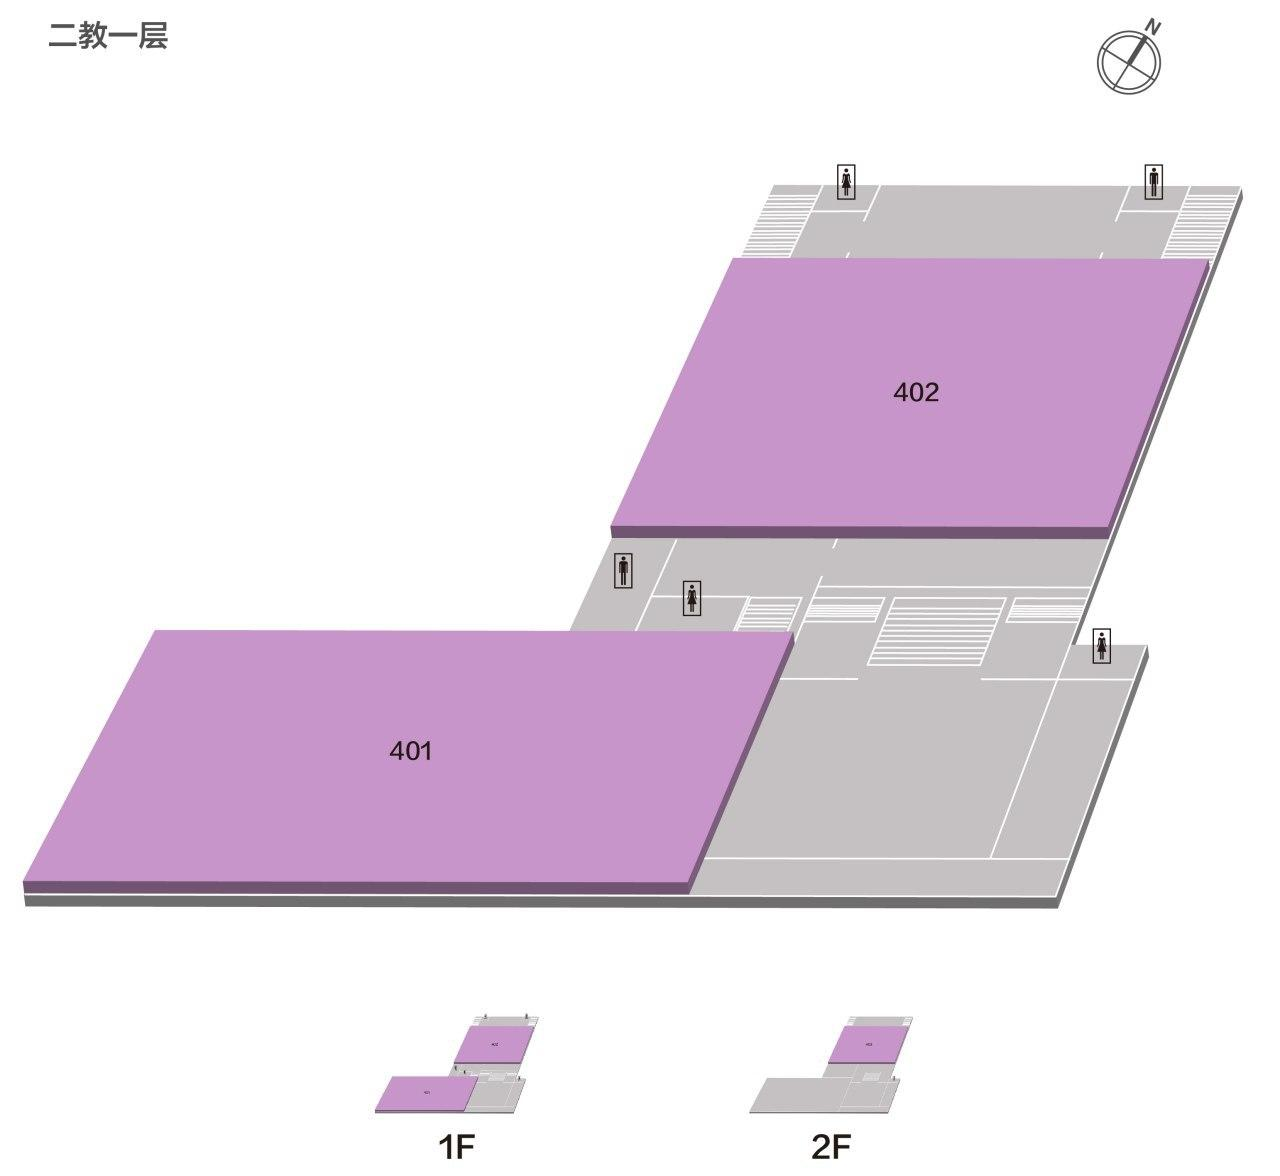
\includegraphics[width=\linewidth]{figures/二教一层.jpg}
	第二教学楼一层结构。两张结构图都取自清华大学“学在清华”公众号2018年9月16日的推送\href{https://mp.weixin.qq.com/s/SHW-wviq3NYemcHZBRgi5w}{《解救路痴 | 清华教室最强指南》}。
\end{figure}

\vfill

\paragraph{闲谈}
笔者记得自己在大一的时候在校内的某公众号上看到过一篇推送,做的是清华园校内怪谈集锦。感觉这种奇闻异事应该是又“小五爷园”来发的,不过近来回去搜索历史却并没有搜到相关的文章。想来也有可能是什么群里发出来的链接被笔者看去了吧。
看完之后印象最深的就是二教地下室的传说,因此这番也打算围绕着二教来写。只是当时看的故事如今早已模糊不清,故又到网上搜集了些材料,在此转述出来。
文中除了“空中楼阁说”是笔者自行杜撰之外,其余故事的灵感皆来自搜集的材料。

\begin{figure}[!t]
	\centering
	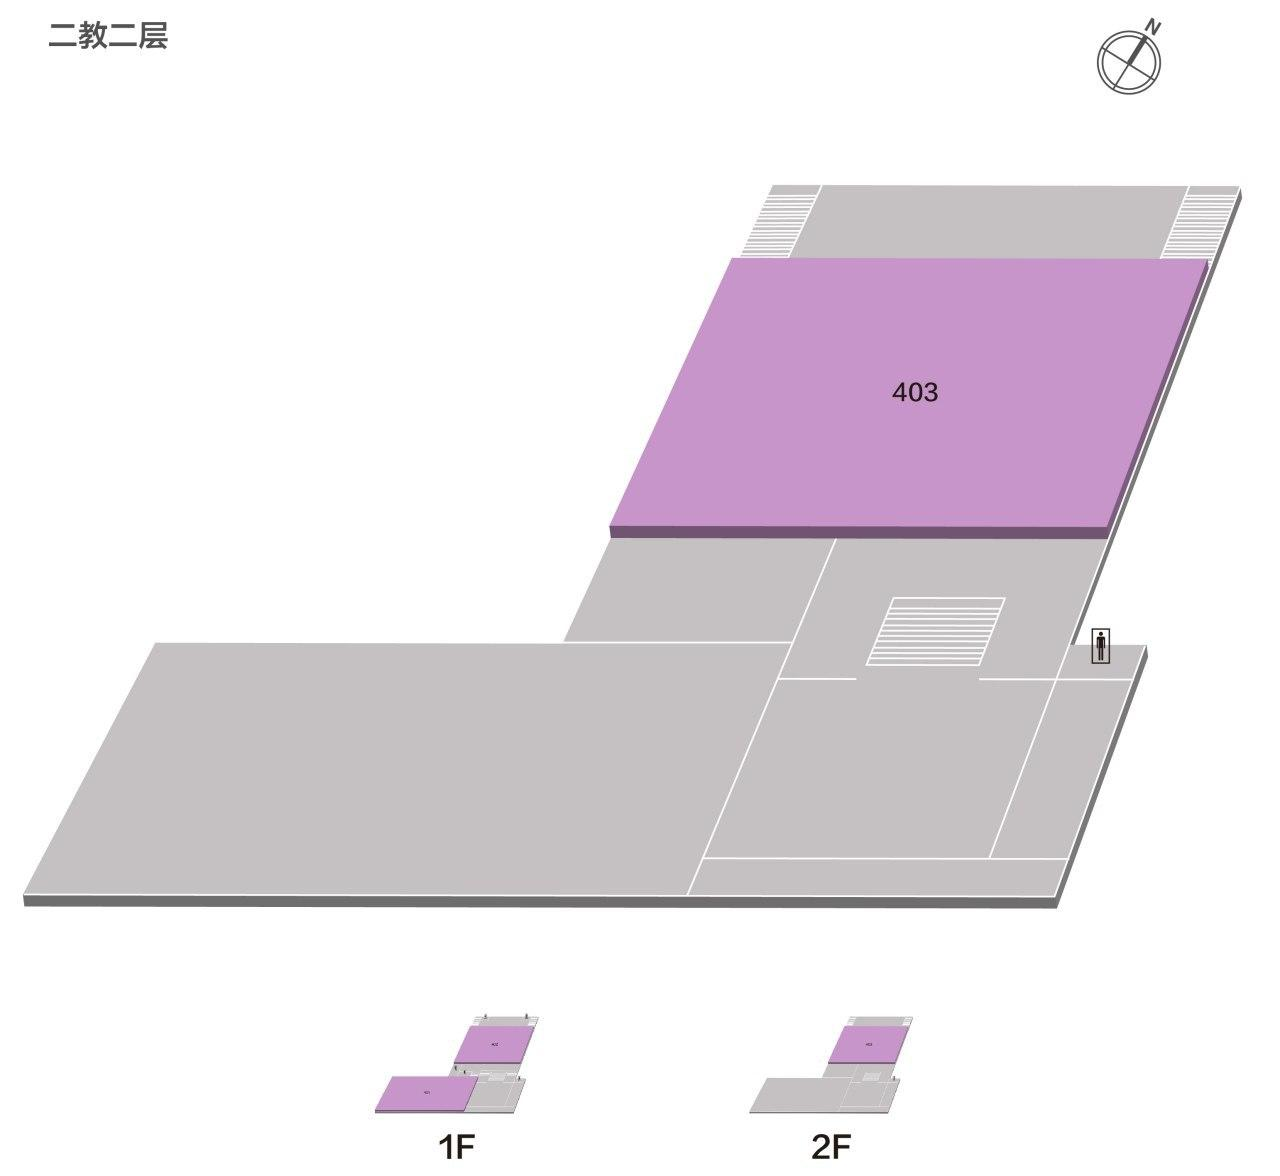
\includegraphics[width=\linewidth]{figures/二教二层.jpg}
	第二教学楼二层结构
\end{figure}

说到二教,其实笔者在二教只上过两门课。
大一下的时候上安宇老师的《大学物理(1)》,线上慕课加线下习题讨论课,每周的习题讨论课就是在二教的403。
403在二楼,从二教的北门进去,上楼梯就是403的后门。记得那是403的前门往里是不开的,貌似是堵死的,出入只能走后门,而且二教也不开放自习,给人感觉很神秘。
之后大二下,罗予频老师的《计算机原理与应用》也是在二教,不过是在402。402就在403的楼下,可以从北楼门由教室后门进,也可以从正楼门由教室前门进。
网上谣传401只能从南门进,但笔者记得当时401和402的前门差不多就对着,从正门是可以进去的。二教的南门笔者也没仔细留意过,感觉好像这个门是不开的吧。
二教的结构图上401的楼上,大概就是传说中404的位置。看维基百科上的介绍说,二教其实是三个教室和一个会议室,所以404的位置可能就是会议室吧。这一点笔者也不确定,从来没有从正门处的楼梯上过二楼,403的前门也出不去,因此不知道那个位置是什么样子的。
404这个编号也很巧,正好是HTTP协议中“资源未找到”(Page Not Found)错误的代码,因此校内也流传着“二教404 Not Found”这个梗儿。

根据公开的校史信息,目前校内六座公共教学楼里,最早建设的第一教学楼落成于1952年,而第二教学楼则建成于1954年,都在建国后,因此日本人实验室的故事毫无疑问是伪造的。
不过日本人的人体实验室大约也并非空穴来风。有些记载显示,侵华日军占领清华园期间,曾占用过图书馆老馆做军事医院,二教这个传说的来源可能与此有关。
此外,在搜集材料的时候,还看到有人提起说,文革期间二教确实发生过一些什么事情,但是笔者却没有找到更详细的记述。
话说到人体实验室,在现在校内西北门西侧,医学院那篇区域,靠近学校边界的一个小角落里,有一排平房,是学校的人体实验室,以前阳光长跑的时候,笔者和J君曾胡碰乱撞跑到过这里。

此外,二教好像是没有地下室的,更不会有地道之类的。
倒是大礼堂的地下,建得很深,还很曲折,仿佛地宫一样。
虽然现在只是个厕所,但不知道过去是不是有考虑过用于防空之类的。

还有一个有趣的事情。
清华的一教到五教的牌子上写的都是“第几教\textbf{学}楼”,而六教的牌子上写的却是“第六教\textbf{室}楼”,并不一致。

有人曾务实地分析二教不开放自习的原因,猜测应该是这里离教学区、宿舍区、食堂都很远,来这里自习的时空成本很高,因此来的人少;二教又是阶梯教室,不适合自习,于是就只开放了一教和清华学堂,而没有开放二教。笔者亦以为然。
说到这里,笔者还曾遇到过某个死脑筋在一教自习的人。
笔者大四时选了个课,是后八周的课。周五早上去一教102上课的时候,总能看到个人在那里自习,然后等到7点50多快上课的时候,就会收拾东西离开。
笔者在这里就不去探究为何要大清早的跑到离宿舍区老远的一教来自习了,而是讨论下另一件事情。
按理来说,上过几周课之后,榆木脑袋用它的朽木脚趾也能想到,一教102周五第一节是有课的,为什么仍然要死脑筋地就在一教102早自习而不能换间教室呢?这个人一直到最后一周的周五都保持着这种令人迷惑的行为,即不知道什么时候,总之很早就来到一教102自习,然后等到7点50多教室里快要上课的时候再离开。笔者想不通。

园子老了,就会有各种各样的故事,清华园的怪谈也不仅仅局限于第二教学楼,其他神秘的、有故事的地方也还有很多,比方说,二教对面的清华学堂。
就笔者的个人感觉来说,清华学堂实在比二教更加阴冷。笔者就去过几次清华学堂,最早是C君引笔者进去转了一圈;后来是大四试选了叉院的《密码学基础》,在那里上了几周课,后来退了。每次进去都觉得——很冷,即使是夏天,也会觉得浑身发冷;冬天便更甚,总觉得仿佛没有开暖风一样。实在不敢想象C君他们学堂班的同学是怎么在里面上过四年的课的。
再一个流传甚广的传说之地就是六教了。传闻六教是建在乱葬岗上的,结果去年六角北边的出土文献保护中心和新土木馆的施工地点还真挖出了明清古墓,也堪称传奇了。
还有传闻说六教东边的什么第十三个杨树的异闻的。顺便一提,据说六教东边、主楼后边、综体前边的这片小树林,平时就是鸳鸯夜戏的地方,不过笔者没有亲自考证过。
网上还流传万泉河乃阴气之源,而28号楼南侧,横跨万泉河的那座小桥处——其实就是之前小桥烧烤的地方——是阴气汇集之地,故设置了小桥烧烤店,引入些烟火气,驱驱阴气。
不过如今小桥烧烤也拆除这么久了,好像也没有发生什么鬼魅害人的事件。
笔者还看到有人提及主楼425也有些奇异的传说,不过笔者没有找到具体的故事,故在此不表。

\nocite{ClassroomBuilding2_Leg1,ClassroomBuilding2_Leg2,ClassroomBuilding2_Info1_THU,ClassroomBuilding2_Info2_Wikipedia,ClassroomBuilding2_Anal1,ClassroomBuilding6_Leg1,WanquanRiver_Leg1}
\putbib


% TODO: 请Oran作跋

\end{document}
